\chapter{Classification}
Let's start this chapter saying what means implementing a classifier.
This matches a variety of different pattern recognition problems that requires you to take decisions about what you are actually seeing in a picture.
So basically, it is when you have to determine what the object present in the picture represents.
And in order to do it you need to use the features of the appearance of the object and determine the category it belongs to.
Also, in the previous chapter, we saw how pedestrian detector was working at that level. 
We just focus mostly on the feature extraction part and not really too much about the classifier itself, 
but what we did for the history of gradients was exactly to determine what were the silent elements 
that could characterize the shape of a human body. 
But there are tons of scenarios in which things like that are useful, some examples are:
\begin{itemize}
    \item In a supermarket implement a system that recognizes vegetables;
    \item At the gate of your house, restrict the access to specific subjects or cars;
    \item At the entrance of a parking lot determine the category of the entering vehicle;
    \item On a robot, look for objects (doors, humans, obstacles).
\end{itemize}
The first element that we need to understand is actually what is a class.
In a general representation a class is nothing but a set of properties, which can consist in colors, textures, patterns \dots
\\\textit{NB: Objects or some parts of objects can be overall represented under the same umbrella over class.}
\\
A class is typically made up of a set of descriptions provided by observing a large number of examples and classes contain items that share similar properties
Basically, goal of a classifier is to take an object as input and to output the class label it belongs to.
So, we typically start from an input image and it can be taken as a whole or it can be segmented in advance. 
For example, if we want to detect the pedestrians in a scene, it could be an option to run a detector in a way that I can isolate the portion of the screen where things are moving, and I'm expecting that pedestrian are moving.
So I can isolate some segment, so areas, which are potentially good for being a pedestrian (just a simplify example).
Or again, I can do a segmentation of the picture filtering out the colors that do not mach the range of color of the skin.
To sum up, segmentation is an option, a step that can be conducted and otherwise I'm proceeding with one of the most relevant steps in the classification, which is the extraction of features.
\\
Extraction of features means that i'm looking to the history of the gradients which are being located in a certain portion of the segment of the picture itself.
Basically we compare the picture vector with the feature vector that I used for the training phase, where the feature vector is the one that describes what I have extracted from the picture.
So I feed this information into the machine that will start reasoning about what it sees as an input and in the end it would return an output.
But here we are doing a process called recognition, which is an additional step forward to the detection.
\section{The classification process}
Just to wrap up a little bit, The classification process can be summarize in 4 steps:
\begin{itemize}
    \item Segment the image if necessary;
    \item Extract the features;
    \item Use the feature vector to feed a classifier;
    \item Output a label.
\end{itemize}
In order to make the concept simple let's take as example children. They learn new things by examples, so, to distinguish a dog from a cat they rely on observing samples of these two animals. 
We realize they have learned the concept by the time they see a new sample and they’re able to recognize it.
Basically, teaching a computer works the same way.
Without entering in the realm of NN, let's take a generic recognition system. It requires a high number of examples in order to be able to distinguish across different classes.
Indeed, the creation of a dataset is the most tough job, moreover the dataset need to be annotated (labelled).
\subsection{Subject to failure}
Machines may take days or weeks in order to learn concepts. However, they still tend to fail because of lack of data, wrong annotations, occlusions, perspective, similarity among classes \dots
Systems typically are not able to generalize, so for example, you have classifiers that are mounted on cars which are very robust in detecting cars, but only from a precise perspective.
But what is the pipeline overall over classifier?
\begin{figure}[h]
    \centering
    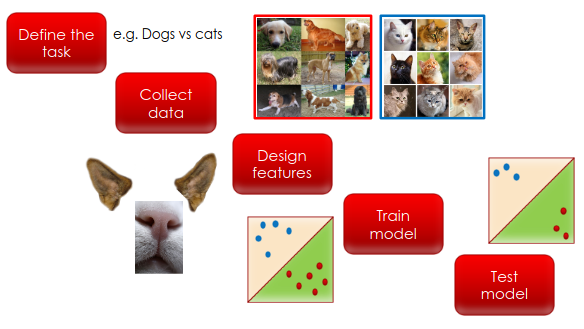
\includegraphics[scale=0.6]{Figures/PipelineClassifier.png}
\end{figure}
So basically, once the model is trained and has found the boundary that separates the two classes, if we put a cat image it falls on the right part, while if it is a dog one it falls on the left area. But if th points fall around the line it can be that we are making mistakes.
In this case we would reduce the performance of our classifier. From this we obtain that one of the simplest problems in classification is regression.
\section{Regression}
To explain it we take an example as a use case. We are trying to predict the share price of a company that is about to go public.
So, if we want to go public, what is the expected price? We need to have some examples in order to determine what is the shape, the inclination of this line in terms of slope and intercept.
And we're doing it by looking at other companies similar to ours, at their revenue and the corresponding share price(features).
In this way we create the training set that will be useful for us to define the parameters of the line,
By looking at the line we have we could try to predict a new pair of coordinates and then compare with the real point. This process is the simplify version of the creation of a loss function.
Meaning that we are trying through this loss function to understand how close we grt to our ground truth.
\begin{figure}[h]
    \centering
    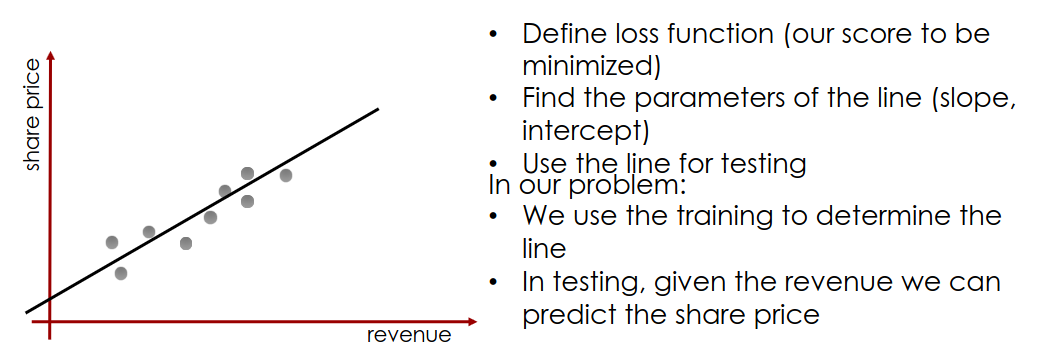
\includegraphics[scale=0.4]{Figures/Regression.png}
\end{figure}
More formally,
\begin{itemize}
    \item We have a set of training samples $D=\{Z_1, Z_2, …, Z_n\}$;
    \item We have an unknown process $P(Z)$;
    \item And a loss function $L(f,Z)$ where $f$ is the decision function;
    \item In supervised learning each example is a pair $Z(X,Y)$ where:
        \begin{itemize}
            \item $X$ contains the features for that sample;
            \item $Y$ is the known/expected output;
            \item $f$ takes $X$ as an argument and outputs something in the range of $Y$
        \end{itemize}
    \item Loss function defined as:\[ L(f, (X,Y))=||f(X)-Y||^2\]
\end{itemize}
Overall, a classifier can be schemed down in a very, very, very simplistic way to a function like that. So it tries to minimize the difference between the estimate and the corresponding ground truth.
So far we were talking about binary classification but usually we have something which is a multi class detector and needs a more complex loss function.

It tends to not have very sharp boundaries and the function which is typically used is a lot like a conditional log-likelihood them.
Very quickly, we are moving into the probabilistic domain, in which we say that $f_i(X)$ estimates $P(Y=i|X)$, where $Y$ is a class (finite integer) and the loss function is the negative conditional log-likelihood.
Of course we have the constraint that the entire sum of all these functions are mapped with one. \[f_Y(X)>= 0\] \[\sum_{i}^{}f_i(X)=1\] 
Another way for multi class classification is in the world of unsupervised learning, we are talking about clustering. In this case we do not provide any prior knowledge to the classifier about the input data.
We feed samples into the algorithm and he progressively adjust the positioning of the different clusters and associates the different input in blind. Basically, through clustering the space is partitioned in regions centered around a prototype (centroid).
\\
As an output you may have correct or incorrect detection, in a binary classification problem you can have True positive (hit), True negative, False positive or False negative (miss).
\\
If we have a classifier for cat and dog and feed a bird into the system we obtain that the likelihood is extremely low, so we can implement a so-called reject option, in which the system prefers to just reject the examples and not give an answer. 
\subsection{The ROC curve, Precision and Recall}
The ROC (Receiver Operating Characteristic) curve is a plot of the True Positive Rate vs the False Positive Rate. Each setup of the system is a point in the ROC space.
\begin{figure}[h]
    \centering
    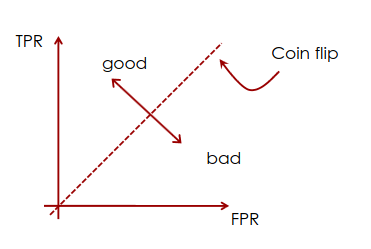
\includegraphics[scale=0.5]{Figures/ROC.png}
\end{figure}
We basically would like to have something which stays above the coin flip. More precisely we want something that minimize as much as possible the contributions along the x axes and instead maximizes the contributions on the TPR axes.
\\(\textit{NB: If the performance is on the line or under you better use a coin to classify.})
Given TRP and FPR we can define other two basic parameters which are the precision and the recall.
\\Precision: $TP/(TP+FP) = hit/(all retrieved) \Rightarrow$ probability that a randomly selected elements is relevant.
\\Recall: $TP/(TP+FN) = hit/(hit+miss) \Rightarrow$ probability that a randomly relevant element is retrieved in the search.
If we extend the concept to more complex scenario where we have multiple classes, we can create a confusion matrix. 
\section{The face detection problem}
Once I have identified the significant features for the object that I'm looking for, I can take some samples and train the classifier.
If I’m looking for faces the problem can be to find all faces (so binary detection), or find Bart-Lisa-Homer-Marge (recognition).
The two scenarios are very different and involve the application of different algorithms.
\\Let's talk about the Viola-Jones algorithm, that is probably the most widespread face detector also in terms of implementation because it is faster, quite robust and available in openCV.
The goal was to implement a robust classifier using simple binary features.
So the classifier is constructed using 14 Haar-like features:
\begin{figure}[h]
    \centering
    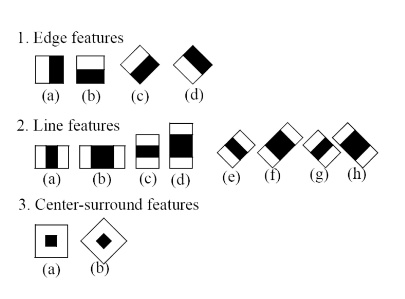
\includegraphics[scale=0.7]{Figures/ViolaJones.png}
\end{figure}
Basically, the sum of the pixels within the white rectangles are subtracted from the sum of pixels in the black rectangles.
Rectangle features can be computed easily using an intermediate representation for the image called the \textit{integral image}.
\[ii(x,y)=\sum_{x'<=x, y'>=y}^{}i(x', y')\]
It is an intermediate representation of the image in which we are defining a single value $ii(x,y)$ that represents the contribution of the pixels before that location.
\begin{wrapfigure}{l}{0.5\textwidth}
    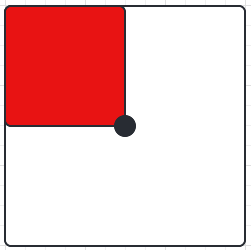
\includegraphics[width=0.5\linewidth]{Figures/IntegralImage.png}
\end{wrapfigure}
So, for example, if we want to compute the integral image at the black point, we just need to dum up the contribution of the pixels in the red area.
\\This makes the computation faster, if we start scanning the image from the top left corner and we go to the bottom right corner, we can compute the integral image in a single pass.
At any shift we can rely on the previous summation, add the last contribution and so on and so forth.
\\Remember that we are evaluating binary features, so we are looking at the difference between the sum of the pixels in the white area and the sum of the pixels in the black area.
\begin{figure}[h]
    \centering
    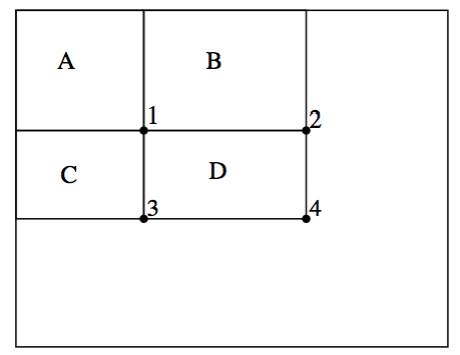
\includegraphics[scale=0.4]{Figures/IntegralImage2.png}
\end{figure}
\\So, looking at the image above, we can compute the sum of the values in D in the following way.
Knowing that: 
\[1 = A,\quad 2 = A + B,\quad 3 = A + C,\quad 4 = A + B + C + D\]
We obtain that the sum of the values in D is $0$:
\begin{equation}
    \begin{split}
        D & = 4 - (A + B + C) \\
        D & = 4 - (2 + C) \\
        D & = 4 - (2 + 3 - 1) 
    \end{split}
\end{equation}
\subsection{Recursion}
Using the following recursions, the integral image can be computed over the entire image in one single pass:
\[s(x,y)=s(x,y-1)+i(x,y)\]
\[ii(x,y)=ii(x-1,y)+s(x,y)\]
where $s$ is the cumulative row sum.
\\I can basically rely on what has been computed up to the previous role and then add the last contribution.
\\
\\
Now we go into the detail of the classifier. In literature we have a lot of different classification algorithms. We have deep networks which are the most popular nowadays, but there is a time when there were other algorithms which are still fine.
Usually the most popular algorithms are:
\begin{itemize}
    \item SVM (Support Vector Machine);
    \item Artificial Neural Networks such as Multi Layer Perceptron or Radial Basis Function;
    \item Boosting algorithms such as AdaBoost;
\end{itemize}
The paper that professor is referring, Viola-Jones, is actually based on the AdaBoost algorithm (adaptive boosting classifier), so now let's see how it works.
\subsection{AdaBoost}
The AdaBoost algorithm is a boosting algorithm that combines multiple weak classifiers to create a strong classifier.
They decided to create a final function $f$, that we recall it to be what we want to get in our classifier, as a linear combination of the weak classifiers $h_i$.
The weak classifiers are trained sequentially, each new classifier is trained on the misclassified samples of the previous classifiers.
So in terms of output, what we have is a sum of different contributions, where each contribution is weighted by a coefficient $\alpha_i$.
After defining the threshold, it will return either $1$ or $-1$.
\[
f(x)=\sum_{i=1}^{T}\alpha_ih_i(x)    
\]
where $h_i$ is the weak classifier and $H(x)=sign(f(x))$ is the final strong classifier.
\[h_i(x)=\begin{cases}
    1 & \text{if } f_i(x) \textit{threshold} \\
    -1 & \text{otherwise}
\end{cases}\]
So, if it returns $1$ it means that somehow the object is relevant, otherwise it means that I don't find this element as relevant.
\[f_i = Sum(r_{i, white}-Sum(r_{i, black}))\]
More formally, given a set of points $(x_i,y_i), i=1\dots m,$ with $y = \pm1$, and a set of weights all set to the same value $D_1(i)=1/m$, what we do is to evaluate the features and try to find the configuration of the classifiers that minimizes the error.
So, we try to minimize the sum of the weights of the misclassified samples.
\[h_t = argmin_{h_j \in H} {\epsilon_j}=\sum_{j=1}^{m}D_t(i)I(y_i \neq h_j(x_i))\]
where $I$ is the indicator function(binary).
If error is less than $0.5$ we can use the classifier, otherwise we can discard it.
Now we need to choose the weight of the classifier and from here we start to update progressively the system, we adjust the learning procedure for specific features inside a specific image.
\[\alpha_t = \frac{1}{2}log(\frac{1-\epsilon_t}{\epsilon_t})\]
\[D_{t+1}(i) = \frac{D_t(i)e^{(-\alpha_ty_ih_t(x_i))}}{Z_t}\]
where $Z_t$ is a normalization factor.
\textit{NB: Samples that are more difficult to classify will have higher weight in the next iteration.}
As we say before, the final output is the summation of the different weak classifiers with the corresponding weight and the sign which basically tell us if the object is relevant or not from a graphical perspective.
\[
H(x)=\textit{sign}(\sum_{t=1}^{T}\alpha_th_t(x))
\]
Let's do a quick recap\dots
\begin{itemize}
    \item In AdaBoost the combination of the weak classifiers improves the speed of the classification process and in the algorithm proposed by Viola and Jones, classifiers are used
in cascade, further reducing the computational complexity;
    \item The goal is to quickly remove false negatives and focus on the positive samples.
\end{itemize}
Remember that in face detection, basic features can be used to exclude non-faces.
The output of the first classifier is used to trigger the second one and at each stage the negatives are rejected.
Let's make an example, if we have a face detector and we have a face in the image, the first classifier will check if he can find a symmetry in between the left and right part of the window, if it doesn't find it, it means that at least we have not a frontal face. Then it discards all the windows that he checked so that the second classifier will not waste time on them and has less tasks to perform.
\begin{itemize}
    \item In the cascade, binary features are evaluated on training images of equal size (24x24pix);
    \item During the training stage, the boundaries of the classifiers are learned;
    \item During the testing phase, the learned classifiers are used to evaluate unknown samples;
    \item Images are not scaled at 24x24, so a multi-scale analysis must be conducted (at the feature level $\Rightarrow$ fast by considering the type of detector [binary + integral image]);
    \item In case of multiple detections at different scales, windows are averaged.
\end{itemize}
For what concerns the complexity we must say that it depends on the number of classifiers, the number of levels in the multi-scale analysis and the sampling distance between the windows.
